% !TeX root = ../build/main.tex

Below, we detail the components of the architecture that collectively support the operation and management of the voting system.

\begin{figure}[h]
	\centering
	\fbox{
		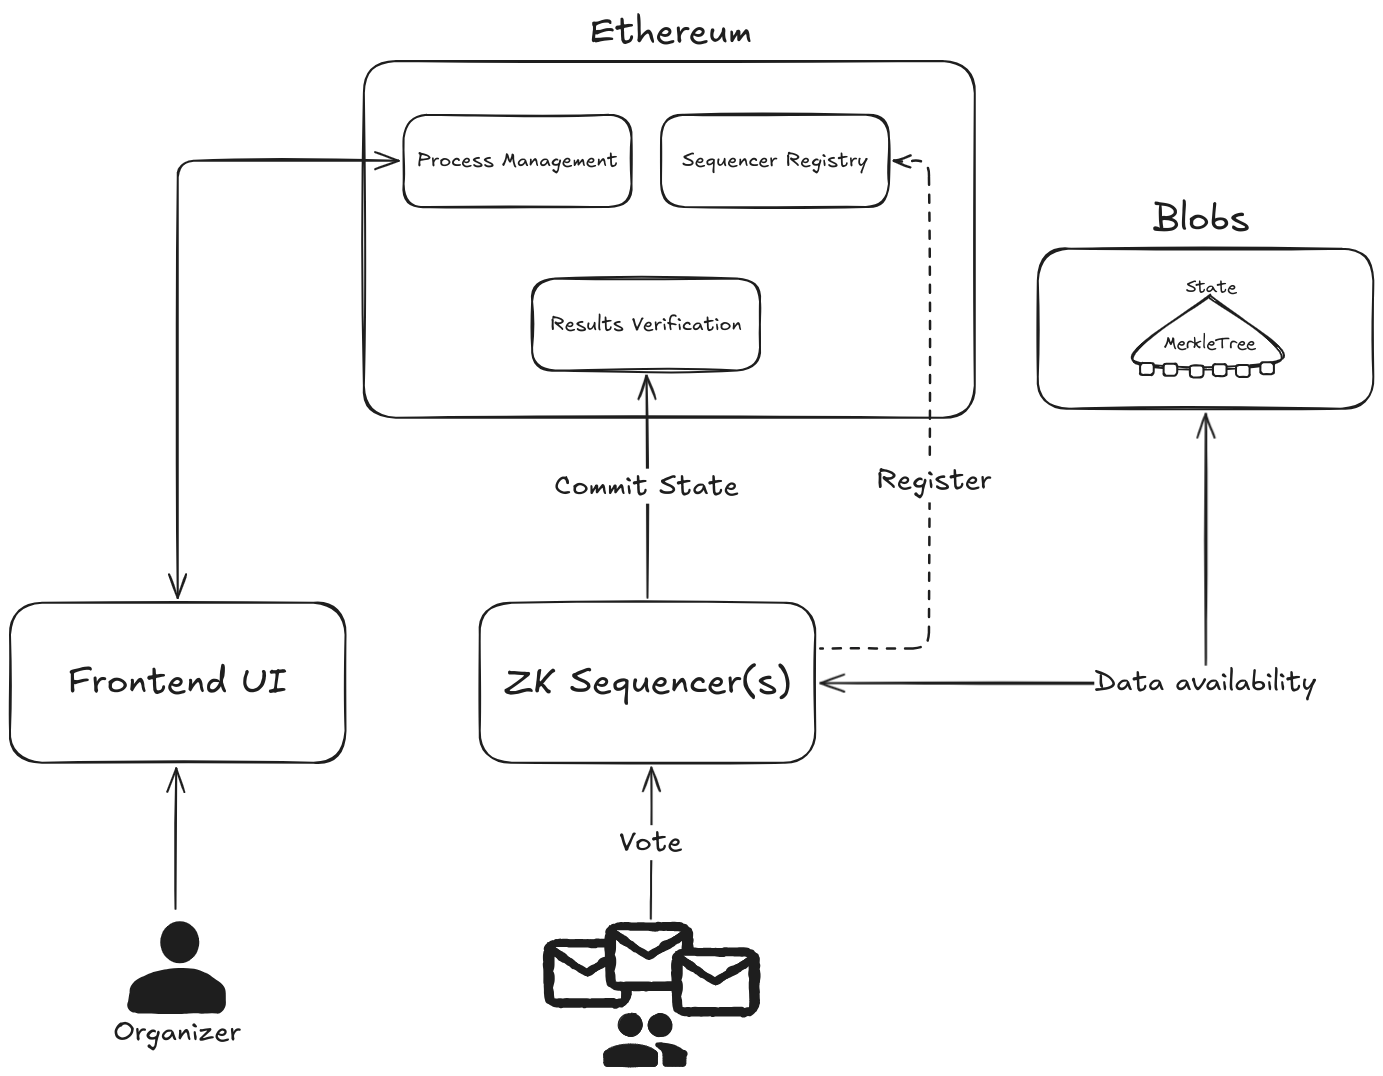
\includegraphics[scale = 0.2, draft = false]{\figs/architecture.png}}
\end{figure}

\subsection{Ethereum}

An Ethereum compatible network is used as the source of truth for the voting system. By leveraging an EVM blockchain, the process management ensures that all transitions are immutable and verifiable by all participants. To this end, we implement several smart contracts.

\begin{itemize}
	\item \textbf{Process Management}: Responsible for the lifecycle management of voting processes. It includes the initiation, monitoring, execution, and closure of voting events.
	
	\item \textbf{Results Verification}: For each voting process, this smart contract maintains the integrity of the cast votes and process lifecycle. It verifies that each state transition committed by a ZK sequencer adheres to the predefined rules.
	
	\item \textbf{Sequencer Registry}: This smart contract keeps track of the existing available sequencers, stores the collateral to ensure good behavior, and it's used to coordinate the distributed key generation when a new Process is created.
\end{itemize}

\subsection{Sequencer}

The Sequencer is a specialized component designed to handle the voting process using zero-knowledge proof mechanisms. It ensures that all transactions related to this process are validated and sequenced. The Sequencers periodically commit the state of the voting process to Ethereum.

\subsection{Frontend User Interface}

The user interface serves as the primary interaction layer for voters and organizers. It provides tools and functionalities needed by organizers to set up, manage, and oversee elections. This interface simplifies the complexities involved in managing a decentralized vote.

\subsection{Data Availability}

For each voting process, the system needs to keep track of the current State Merkle Tree, which contains all information of such processes. A public data availability layer, ensures that all state transitions are available and verifiable and allows the participation of multiple sequencers within the same voting process.